This Section explains the method and principles used for the system evaluation processes, measuring and comparing the performance (latency, in seconds, and throughput, in rows/second) of reading and writing Iceberg and Delta Lake tables on \gls{HopsFS}. Those operations are conducted respectively on the PyIceberg-based system, integrated in this thesis work, and on the Rust-based system, implemented in a related work \cite{manfrediReducingReadWrite2024}.

\subsection{Evaluation process - RQ2 - Iceberg vs. Delta Lake}
\label{subsec:eval_process_iceberg_delta}
This evaluation process will follow a sequential approach described in Figure~\ref{fig:method_comparison}. Each step of this process is related to one of the \glspl{G}7-9 associated with the \gls{RQ}2 in Section \ref{sec:intro_goals}. The relationships between each process activity and \glspl{G} are here explained:
\begin{enumerate}
    \item \textbf{Identify related work}: this activity is requisite to fulfill \gls{G}7, identifying the related work that includes comparative performance comparisons.
    \item \textbf{Analyze related work results}: this activity maps perfectly to \gls{G}7, analyzing the results coming from the related work identified in the step above.
    \item \textbf{Uniformize results to metrics}: this activity is requisite to fulfill \gls{G}8, uniforming results of related work's experiments according to previosuly defined metrics, i.e., latency, measured in seconds, and throughput, measured  in rows/second.
    \item \textbf{Visualize results}: this activity maps perfectly to \gls{G}8. It takes as input also Iceberg experiments results (\gls{D}1-partial), visualizing thus the experiments' result according latency, measured in seconds, and throughput, measured in rows/second. This activity generates \gls{D}2, the comparative experiments results complemented with tables and histograms, presented in Chapter \ref{ch:results_and_analysis}.
    \item \textbf{Analyze results}: this activity maps perfectly to \gls{G}9, analyzing and interpreting the results delivered in \gls{D}2. This activity contributes to \gls{D}3, generating the comparative analysis of the experiment results, presented in Chapter \ref{ch:results_and_analysis}.
\end{enumerate}
\begin{figure}[!ht]
    \begin{center}
    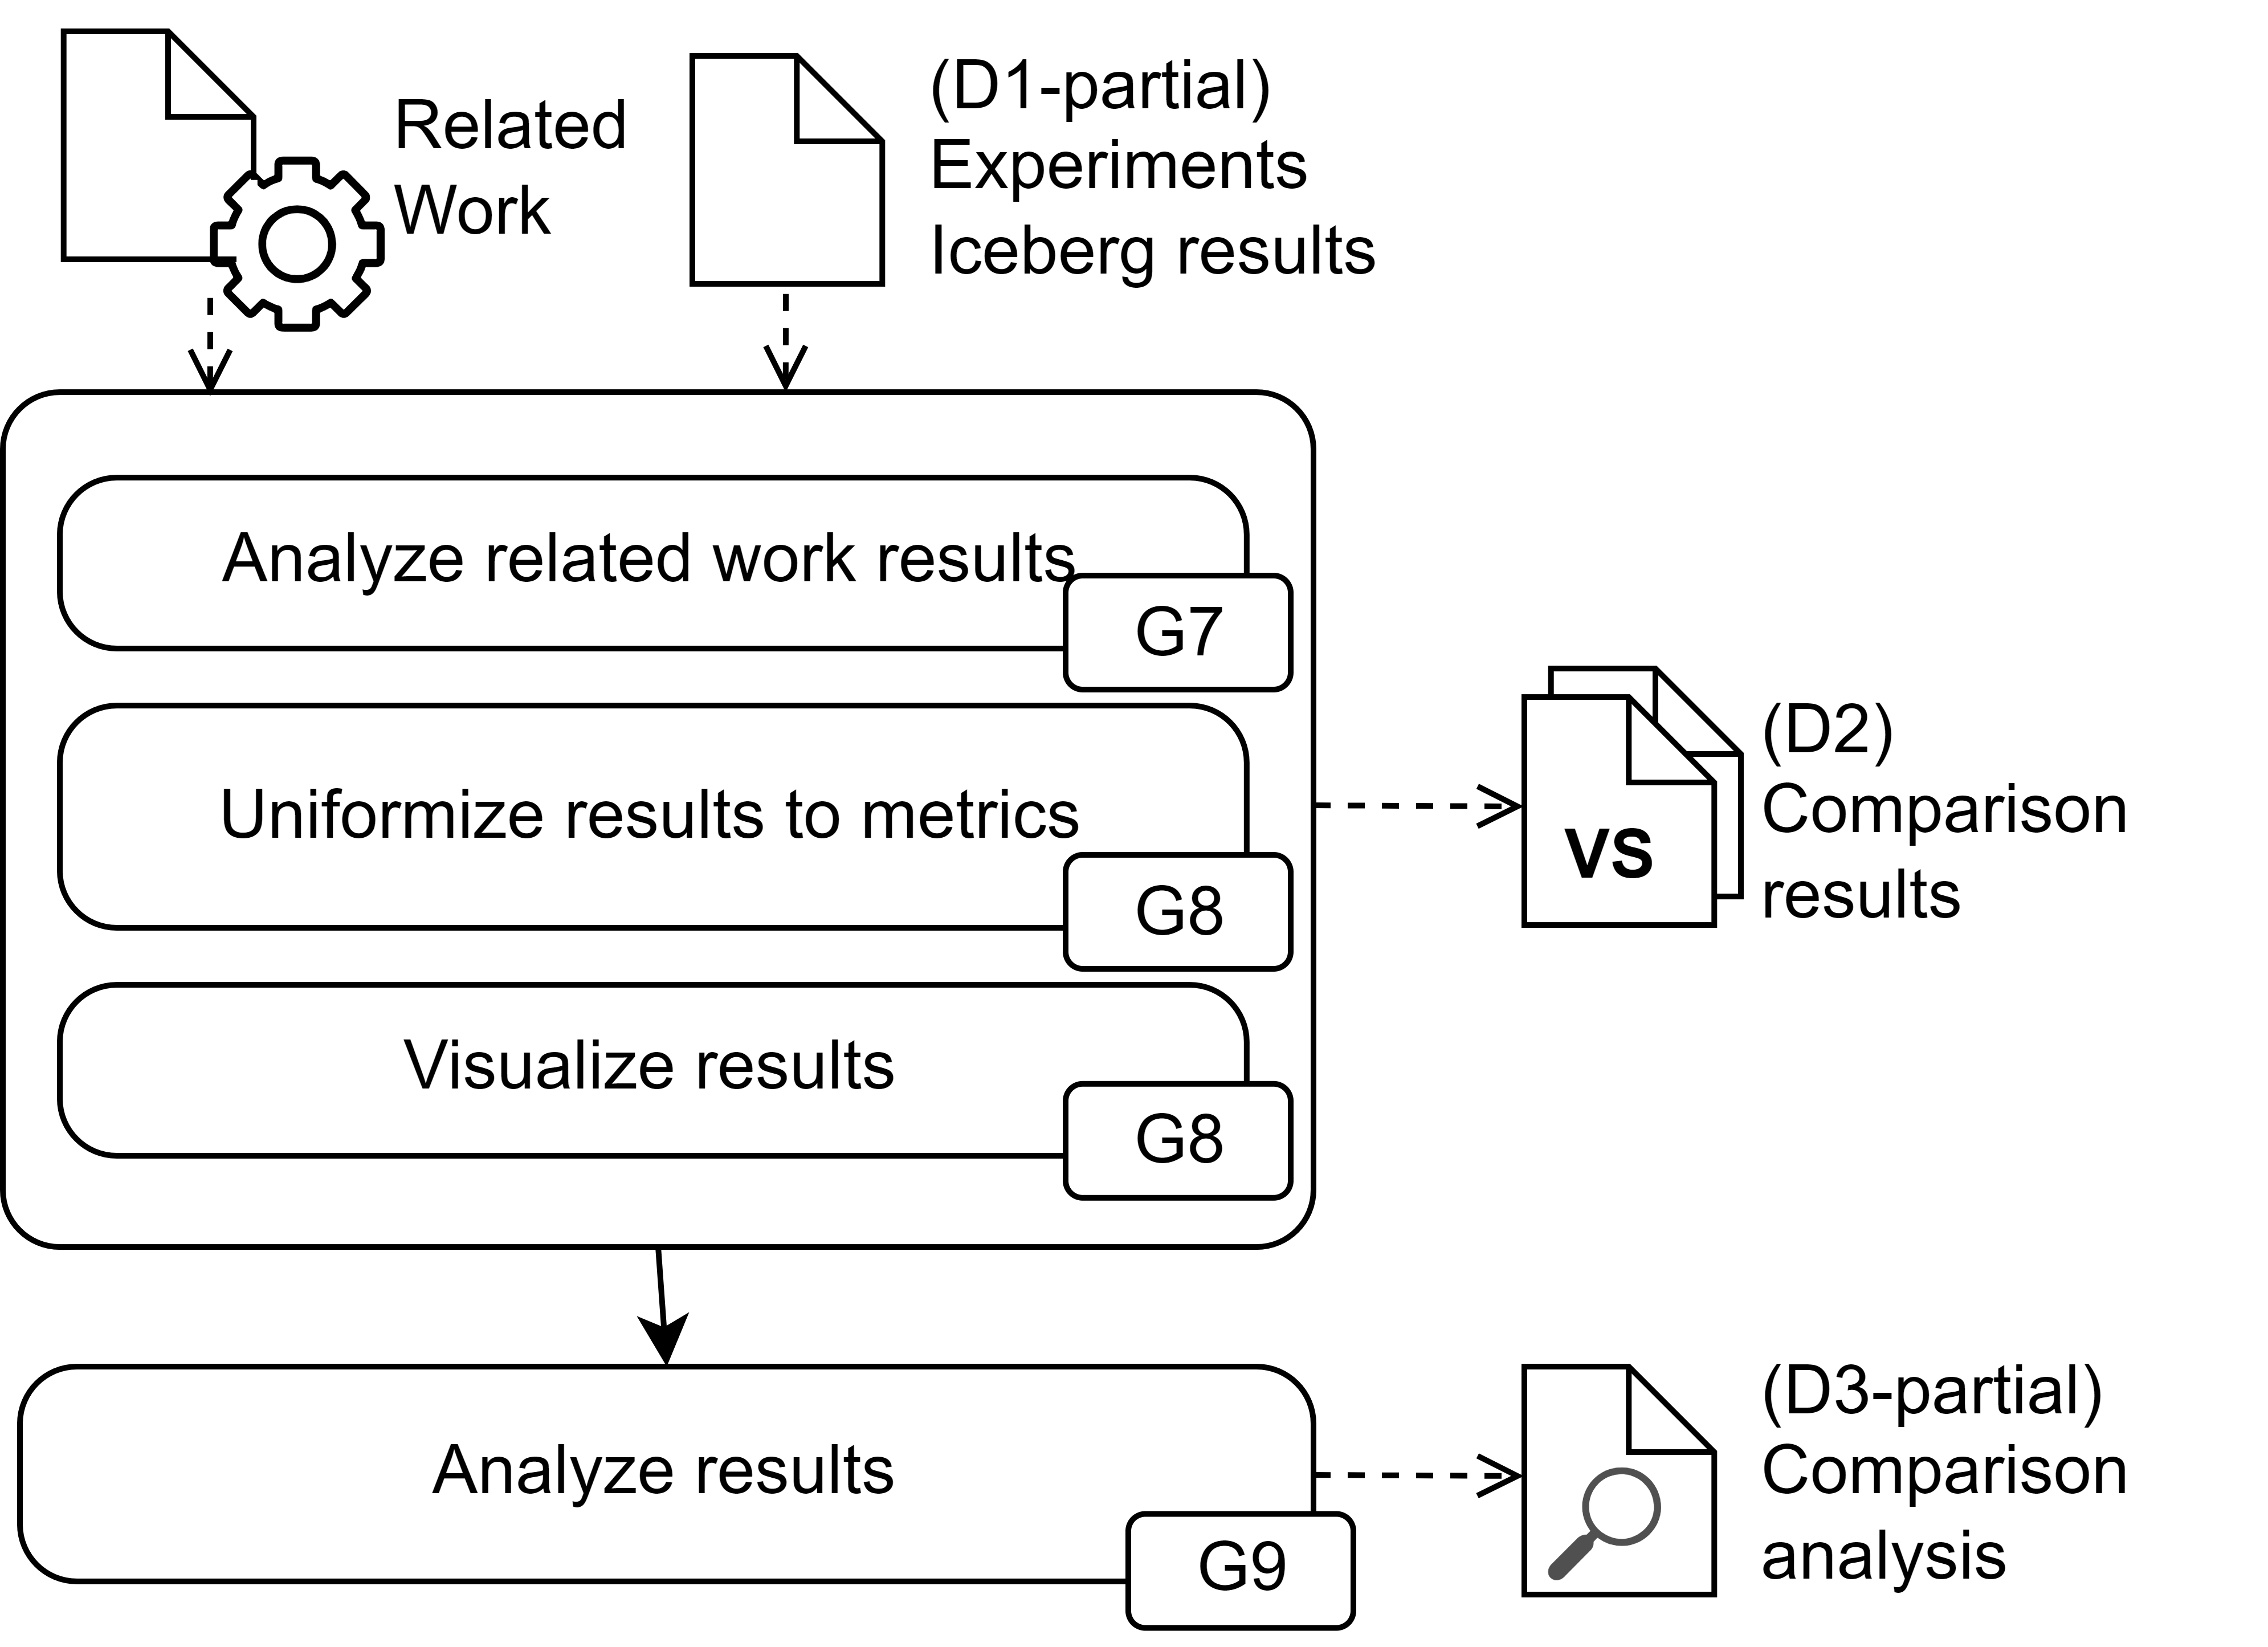
\includegraphics[width=0.8\textwidth]{figures/3-method/method_comp.png}
    \caption[System evaluation process - Iceberg vs. Delta Lake]{Diagram of the system evaluation process partially answering \gls{RQ}2. Each activity is associated to specific \gls{G}. The process produces two \glspl{D}, the comparative expertiments results (\gls{D}2) and a comparative results analysis (\gls{D}3-partial).}
    \label{fig:method_comparison}
    \end{center}
\end{figure}